\documentclass{article}

\usepackage{graphicx}
\usepackage{tikz}
\usepackage{tikzsymbols}
\usetikzlibrary{calc,patterns,shapes.geometric}
\pagestyle{empty}
\usepackage[margin=0pt]{geometry}
\geometry{papersize={14in,12in}}

\def\centerarc[#1](#2)(#3:#4:#5){\draw[#1] ($(#2)+({#5*cos(#3)},{#5*sin(#3)})$) arc (#3:#4:#5);}

\begin{document}
	\begin{figure}
		\centering
		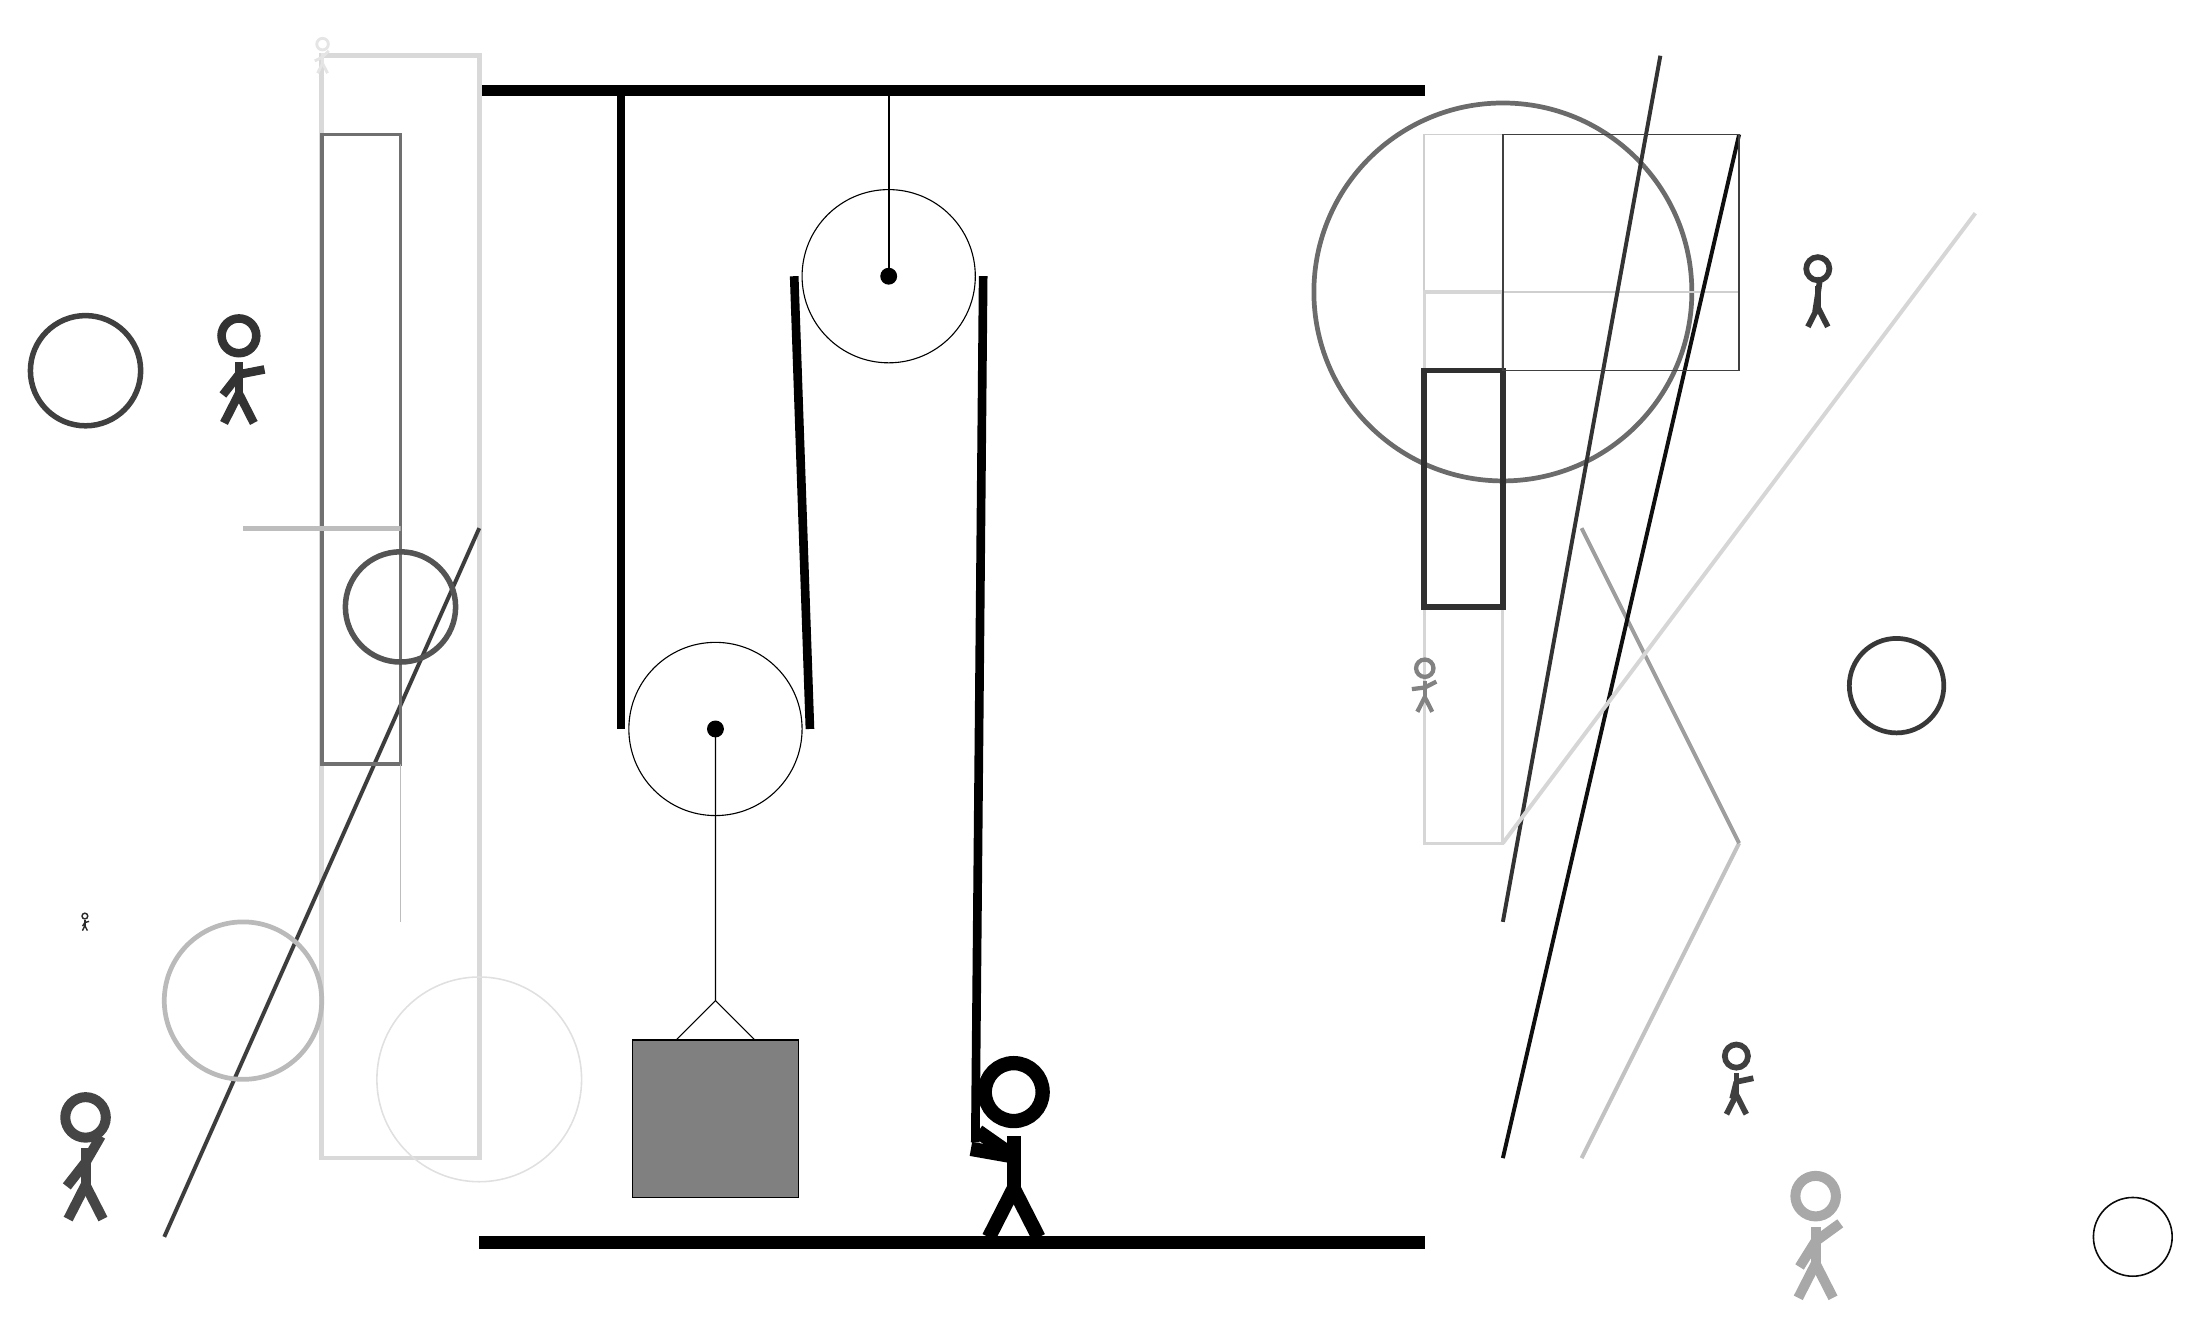
\begin{tikzpicture}
			%%%%% START %%%%%
			
			\draw[fill=black] (-2, 11.5) rectangle (10, 11.625);
			
			\draw [line width=0.6mm, color=black!58](11, 9) circle (2.4);
			
			\node[line width=0.7mm, color=black!34] at (15, -3) {\Strichmaxerl[7][58][36]};
			\draw[line width=0.6mm, color=black!15] (-2, 12) rectangle (-4, -2);
			\draw[line width=0.5mm, color=black!76](-2, 6) -- (-6, -3);
			\draw[line width=0.5mm, color=black!56] (-4, 3) rectangle (-3, 11);
			\node[line width=0.6mm, color=black!10] at (-4, 12) {\Strichmaxerl[2][27][45]};
			\node[line width=0.4mm, color=black!83] at (-7, 1) {\Strichmaxerl[1][58][15]};
			\draw [line width=0.2mm, color=black!12](-2, -1) circle (1.3);
			\node[line width=0.7mm, color=black!78] at (15, 9) {\Strichmaxerl[4][81][82]};
			
			\draw [line width=0.2mm, color=black!96](19, -3) circle (0.5);
			\node[line width=0.3mm, color=black!75] at (14, -1) {\Strichmaxerl[4][76][12]};
			\node[line width=0.5mm, color=black!73] at (-7, -2) {\Strichmaxerl[7][52][60]};
			\draw[line width=0.3mm, color=black!89] (-2, 6) rectangle (-2, 6);
			\draw [line width=0.6mm, color=black!27](-5, 0) circle (1.0);
			\draw[line width=0.5mm, color=black!24](14, 2) -- (12, -2);
			\draw[line width=0.2mm, color=black!19] (10, 11) rectangle (14, 9);
			\draw[line width=0.5mm, color=black!80](13, 12) -- (11, 1);
			\draw[line width=0.4mm, color=black!16] (11, 9) rectangle (10, 2);
			\draw[line width=0.2mm, color=black!26] (-3, 3) rectangle (-3, 1);
			\draw[line width=0.5mm, color=black!38](12, 6) -- (14, 2);
			\draw[line width=0.5mm, color=black!94](14, 11) -- (11, -2);
			
			\draw[line width=0.7mm, color=black!81] (10, 8) rectangle (11, 5);
			
			\node[line width=0.5mm, color=black!49] at (10, 4) {\Strichmaxerl[3][7][27]};
			\node[line width=0.7mm, color=black!80] at (-5, 8) {\Strichmaxerl[6][52][11]};
			\draw [line width=0.7mm, color=black!75](-7, 8) circle (0.7);
			
			\draw[line width=0.6mm, color=black!26] (-3, 6) rectangle (-5, 6);
			\draw[line width=0.2mm, color=black!75] (11, 11) rectangle (14, 8);
			\draw[line width=0.5mm, color=black!16](11, 2) -- (17, 10);
			
			\draw [line width=0.6mm, color=black!78](16, 4) circle (0.6);
			\draw [line width=0.7mm, color=black!67](-3, 5) circle (0.7);
			
			\draw (3.2, 9.2) circle (1.1);
			\draw[fill=black] (3.2, 9.2) circle (0.1);
			\draw[thick] (3.2, 9.2) -- (3.2, 11.5);
			
			\draw (1, 3.45) circle (1.1);
			\draw[fill=black] (1, 3.45) circle (0.1);
			
			\draw (1, 3.45) -- (1, 0.0) -- (0.5, -0.5);
			\draw (1, 0.0) -- (1.5, -0.5);
			\draw[fill=black!50] (-0.05, -0.5) rectangle (2.05, -2.5);
			
			\draw[line width=1.1mm] (-0.2, 11.5) -- (-0.2, 3.45);
			\centerarc[line width=1.1mm](1, 3.45)(180:360:1.2000000000000002);
			\draw[line width=1.1mm](2.2, 3.45) -- (2.0, 9.2);
			\centerarc[line width=1.1mm](3.2, 9.2)(0:180:1.2000000000000002);
			\draw[line width=1.1mm](4.4, 9.2) -- (4.3, -1.8);
			
			\node at (4.7, -1.9) {\Strichmaxerl[10][-35][170]};
			
			\draw[fill=black] (-2, -3) rectangle (10, -3.15);
			
			%%%%% END %%%%%
		\end{tikzpicture}
	\end{figure}	
\end{document}